%beamer

%\PassOptionsToClass{handout}{beamer}

% \newboolean{handoutmode}
% \setboolean{handoutmode}{false}
%\newcommand{\handoutmode}{}

%% LaTeX-Beamer template for KIT design
%% by Erik Burger, Christian Hammer
%% title picture by Klaus Krogmann
%%
%% version 2.1
%%
%% mostly compatible to KIT corporate design v2.0
%% http://intranet.kit.edu/gestaltungsrichtlinien.php
%%
%% Problems, bugs and comments to
%% burger@kit.edu
\ifdefined \handoutmode
\documentclass[18pt, handout]{beamer}
\else
\documentclass[18pt]{beamer}
\fi

\usepackage[T1]{fontenc}
\usepackage[utf8]{inputenc}

\usepackage{../preamble/templates/beamerthemekit}

\usepackage[vlined]{algorithm2e}  %possible: noend, noline, ...
\usepackage{amssymb}
\usepackage{amsmath}
\usepackage{wasysym}
\usepackage{graphicx}
%\usepackage{hyperref}
\usepackage[export]{adjustbox}
\usepackage{wrapfig}
\usepackage{colortbl}
\usepackage{tikz}
\usetikzlibrary{matrix}
\usetikzlibrary{arrows.meta}
\usetikzlibrary{automata}
\usetikzlibrary{tikzmark}
\graphicspath{{images/}}
%\usepackage[colorlinks=true,urlcolor=blue,linkcolor=blue]{hyperref}
\usepackage[outline]{contour}
\usepackage{cancel}
\usepackage[warn]{textcomp}
\usepackage{multicol}
\usepackage{tabularx}
\usepackage{xcolor}
\usepackage{hhline}
\usepackage{environ}
\usepackage{calc}
\usepackage{bm}
\usepackage{xspace} % for \xspace command
\usepackage{varwidth}
\usepackage{csquotes}

\newcommand{\mycomment}[1]{}

%%%% CONFIG

\input{../preamble/config.tex}

%%%% CONFIG END

%\renewcommand{\SS}{\iffontchar\font"1E9E \symbol{"1E9E}\else SS\fi} % SHAME ON YOU, LATEX!
\newcommand{\TM}{\text{$\mbox{}^\text{\tiny TM}$}}
\newcommand{\pluseq}{\mathrel{+}=}
\newcommand{\pp}{\operatorname{++}} 
\newcommand{\mm}{\operatorname{--\mbox{\:}--}}
\newcommand{\minuseq}{\mathrel{-}=}
\newcommand{\asteq}{\mathrel{*}=}
\newcommand{\muleq}{\asteq}
\renewcommand{\mod}{\mathop{\textbf{mod}}} 
\renewcommand{\div}{\mathop{\textbf{div}}}
\newcommand{\N}{\mathbb{N}} 
\newcommand{\R}{\mathbb{R}}
\newcommand{\Z}{\mathbb{Z}}
\newcommand{\E}{\mathbb{E}}
\renewcommand{\P}{\mathbb{P}}
\newcommand{\BB}{\mathbb{B}} % \B already exists
\newcommand{\NP}{\ensuremath{\mathcal{N\hspace{-1.5pt}P}}}
\newcommand{\Oh}[1]{\mathcal{O}\!\left(#1\right)}
\renewcommand{\O}{\mathcal{O}}
\newcommand{\Om}[1]{\Omega\!\left(#1\right)}
\newcommand{\Th}[1]{\Theta\!\left(#1\right)}

\newcommand{\realTilde}{\textasciitilde\xspace}
\renewcommand{\qedsymbol}{\textcolor{black}{\openbox}}

\newcommand{\size}[1]{\ensuremath{\left\lvert #1 \right\rvert}}
\newcommand{\set}[1]{\left\{#1\right\}}
\newcommand{\tuple}[1]{\left(#1\right)}

\newcommand*{\from}{\colon}

\newcommand{\morescalingdelimiters}{   % for proper \left( \right) typography
	\delimitershortfall=0pt  % formerly: 0pt  
	\delimiterfactor=1
}
% todo later
%\delimitershortfall=0pt  % for proper \left( \right) typography
%\delimiterfactor=1

% --- \frameheight constant ---
\newlength\fullframeheight
\newlength\framewithtitleheight
\setlength\fullframeheight{.92\textheight}
\setlength\framewithtitleheight{.86\textheight}

\newlength\frameheight
\setlength\frameheight{\fullframeheight}

\let\frametitleentry\relax
\let\oldframetitle\frametitle
\def\frametitle#1{\global\def\frametitleentry{#1}\if\relax\frametitleentry\relax\else\setlength\frameheight{\framewithtitleheight}\fi\oldframetitle{#1}}

% --- \frameheight constant end ---

\def\·{\cdot}
\def\*{\cdot}
\def\<{\langle}
\def\>{\rangle}


\newcommand{\zB}{z.\,B.\@\xspace}
\newcommand{\ZB}{Z.\,B.\@\xspace}

\newcommand{\ceil}[1]{\left\lceil#1\right\rceil}
\newcommand{\floor}[1]{\left\lfloor#1\right\rfloor}
\newcommand{\abs}[1]{\left|#1\right|}
\newcommand{\Matrix}[1]{\begin{pmatrix} #1 \end{pmatrix}}
\newcommand{\braced}[1]{\left\lbrace #1 \right\rbrace}
\newcommand{\llist}[1]{\langle #1 \rangle}
\newcommand{\Mid}{\;\middle|\;}

\let\after\circ

\newcommand{\entspr}{\ensuremath{\mathrel{\hat{=}}}\xspace}

\def\~~>{\ensuremath{\rightsquigarrow}}  % FuCKING FINALLY! :D

% "something" placeholder. Useful for repairing spacing of operator sections, like `\sth = 42`.
\def\sth{\vphantom{.}}

\def\fract#1/#2 {\frac{#1}{#2}}  % ! TRAILING SPACE is CRUCIAL!
\def\dfract#1/#2 {\dfrac{#1}{#2}} % ! Trailing space is crucial!

\newcommand{\tight}[1]{{\renewcommand{\arraystretch}{0.76} #1}}
\newcommand{\stackedtight}[1]{{\renewcommand{\arraystretch}{0.76} \begin{matrix} #1 \end{matrix}} }
\newcommand{\stacked}[1]{\begin{matrix} #1 \end{matrix} }
\newcommand{\casesl}[1]{\delimitershortfall=0pt  \left\lbrace\hspace{-.3\baselineskip}\begin{array}{ll} #1 \end{array}\right.}
\newcommand{\casesr}[1]{\delimitershortfall=0pt  \left.\begin{array}{ll} #1 \end{array}\right\rbrace}
\newcommand{\caseslr}[1]{\delimitershortfall=0pt  \left\lbrace\begin{array}{ll} #1 \end{array}\hspace{-.3\baselineskip}\right\rbrace}

\def\q#1uad{\ifnum#1=0\relax\else\quad\q{\the\numexpr#1-1\relax}uad\fi}
% e.g. \q1uad = \quad, \q2uad = \qquad etc.

\newcommand{\qqquad}{\q3uad}


\def\indentstring{}
\def\§#1{\def\indentstring{#1}#1}
\def\.{{$\hphantom{\text{\indentstring}}$}}


\newcommand{\impl}{\ifmmode\ensuremath{\mskip\thinmuskip\Rightarrow\mskip\thinmuskip}\else$\Rightarrow$\xspace\fi}  
\newcommand{\Impl}{\ifmmode\implies\else$\Longrightarrow$\xspace\fi}

\newcommand{\gdw}{\ifmmode\mskip\thickmuskip\Leftrightarrow\mskip\thickmuskip\else$\Leftrightarrow$\xspace\fi}
\newcommand{\Gdw}{\ifmmode\iff\else$\Longleftrightarrow$\xspace\fi}

\newcommand{\symbitemnegoffset}{\hspace{-.33\baselineskip}}
\newcommand{\implitem}{\item[\impl\symbitemnegoffset]}
\newcommand{\Implitem}{\item[\Impl\symbitemnegoffset]}


\newcommand{\forcenewline}{\mbox{}\\}

\newcommand{\bfalert}[1]{\textbf{\alert{#1}}}
\let\elem\in   % I'm a Haskell freak. Don't judge me. :P


\newenvironment{threealign}{%
	\[
	\begin{array}{r@{\ }c@{\ }l}
}{%
	\end{array}	
	\]
}


\makeatletter
% Provides color if undefined.
\newcommand{\colorprovide}[2]{%
	\@ifundefinedcolor{#1}{\colorlet{#1}{#2}}{}}
\makeatother



%\pgfdeclarelayer{background}
%\pgfdeclarelayer{foreground}
%\pgfsetlayers{background,main,foreground}

\colorprovide{lightred}{red!30}
\colorprovide{lightgreen}{green!40}
\colorprovide{lightyellow}{yellow!50}
\colorprovide{beamerlightred}{lightred}
\colorprovide{beamerlightgreen}{lightgreen}
\colorprovide{beamerlightyellow}{lightyellow}
\colorprovide{fullred}{red!60}
\colorprovide{fullgreen}{green}
\definecolor{darkred}{RGB}{115,48,38}
\definecolor{darkgreen}{RGB}{48,115,38}
\definecolor{darkyellow}{RGB}{100,100,0}

\only<handout:0>{\colorlet{adaptinglightred}{beamerlightred}}
\only<handout:0>{\colorlet{adaptinglightgreen}{beamerlightgreen}}
\only<handout:0>{\colorlet{adaptinglightyellow}{beamerlightyellow}}
\only<beamer:0>{\colorlet{adaptinglightred}{lightred}}
\only<beamer:0>{\colorlet{adaptinglightgreen}{lightgreen}}
\only<beamer:0>{\colorlet{adaptinglightyellow}{lightyellow}}
\only<handout:0>{\colorlet{adaptingred}{lightred}}
\only<beamer:0>{\colorlet{adaptingred}{fullred}}
\only<handout:0>{\colorlet{adaptinggreen}{lightgreen}}
\only<beamer:0>{\colorlet{adaptinggreen}{fullgreen}}

\colorlet{checkgreen}{green!80}
\colorlet{crashred}{fullred}
\colorprovide{myalertcolor}{red}
\colorlet{alertcolor}{myalertcolor}

\definecolor{kwblue}{rgb}{0.3,0.3,1}
\definecolor{strcolor}{RGB}{48,115,38}

\newcommand{\str}[1]{\shorthandoff{"}\textcolor{strcolor}{\text{"{}#1"{}}\shorthandon{"}}}

\newcommand{\gray}[1]{\textcolor{gray}{#1}}

\newcommand{\MyKwSty}[1]{\textcolor{kwblue}{\textbf{#1}}}
\SetKwSty{MyKwSty}

\SetArgSty{textnormal} % to end conditional italics madness

\newcommand{\MyCommentSty}[1]{\emph{\gray{#1}}}
\SetCommentSty{MyCommentSty}

\SetKwComment{Comment}{// }{}

\newcommand{\LComment}[1]{\Comment*[h]{#1}}
\newcommand{\RComment}[1]{\quad \Comment*[h]{#1}}



\SetKwBlock{KwFunc}{function}{}
\SetKwBlock{KwProc}{procedure}{}
\newcommand{\Function}[2]{\KwFunc({#1}){#2}}
\newcommand{\Procedure}[2]{\KwProc({#1}){#2}}
\SetKwBlock{KwEmptyBlock}{}{}
\newcommand{\EmptyBlock}[1]{\KwEmptyBlock(){#1}}

% Binary operator keywords (small surrounding spaces)
\newcommand{\SetKwBin}[2]{
	\expandafter\newcommand\csname #1\endcsname{\ensuremath{\mathbin{\KwSty{#2}}}}	
}
% Relational operator keywords (bigger surrounding spaces)
\newcommand{\SetKwRel}[2]{
	\expandafter\newcommand\csname #1\endcsname{\ensuremath{\mathrel{\KwSty{#2}}}}	
}
% Directive keywords (trailing space)
\newcommand{\SetKwDir}[2]{
	\expandafter\newcommand\csname #1\endcsname{\ensuremath{\mathop{\KwSty{#2}}}}		
}

\DontPrintSemicolon
%\SetKwSwitch{Switch}{Case}{Other}{switch on}{}{}{else}{}{}

%\newcommand{\SwitchCase}[2]{\KwSty{case} #1 \KwOf\EmptyBlock{#2}}
%\newcommand{\case}[2]{#1:\EmptyBlock{#2}}
\SetKwDir{KwAssert}{assert}
\SetKwDir{KwInvariant}{invariant}
\SetKwRel{KwStep}{step}
\SetKwRel{KwDownto}{downto}	
\SetKwDir{KwArrayOf}{array of\,}
\SetKwDir{KwArray}{array}
\let\KwTo\undefined
\SetKwRel{KwTo}{to}
\SetKwRel{KwOf}{of}
\let\KwInput\KwIn
\let\KwIn\undefined
\SetKwRel{KwIn}{in}
\SetKwRel{KwInto}{into}
\SetKwDir{KwNot}{not}
\SetKwRel{KwIs}{is}
\SetKwRel{KwAnd}{and}
\SetKwRel{KwOr}{or}
\SetKwBin{KwMod}{mod}
\SetKwBin{KwDiv}{div}
\SetKwDir{KwContinue}{continue}
\SetKwDir{KwBreak}{break}
\SetKwDir{KwThrow}{throw}
\SetKw{KwTrue}{true}
\SetKw{KwFalse}{false}
\SetKw{KwThis}{this}
\SetKwDir{KwNew}{new}
\SetKwRel{KwFrom}{from}
\SetKwDir{KwFor}{for}
\SetKwDir{KwEach}{each}
\SetKw{KwProcedure}{procedure}
\SetKw{KwMethod}{method}
\SetKw{KwFunction}{function}
\SetKwDir{KwPointerTo}{Pointer to}
\SetKwData{KwList}{List}
\SetKwData{KwSet}{Set}
\newcommand{\Element}{\|Element|}
\newcommand{\KwListOf}{\ensuremath{\mathop{\KwList \KwOf}}} 
\newcommand{\KwSetOf}{\ensuremath{\mathop{\KwSet \KwOf}}} 
\SetKwDir{KwDispose}{dispose}


\def\|#1|{\text{\normalfont #1}}  % | steht für senkrecht (anstatt kursiv wie sonst im math mode)

% proper math typography
\newcommand{\functionto}{\longrightarrow} 
\renewcommand{\geq}{\geqslant}
\renewcommand{\leq}{\leqslant}
\let\oldsubset\subset
\renewcommand{\subset}{\subseteq} % for all idiots out there using subset

\newcommand{\access}{\text{\textrightarrow}} 
\def\->{\access}

\let\oldemptyset\emptyset
\let\emptyset\varnothing % proper emptyset

\newcommand{\stdarraystretch}{1.20}
\renewcommand{\arraystretch}{\stdarraystretch}  % for proper row spacing in tables

\newcommand{\mailto}[1]{\href{mailto:#1}{{\textcolor{blue}{\underline{#1}}}}}
\newcommand{\urlnamed}[2]{\href{#1}{\textcolor{blue}{\underline{#2}}}}
\renewcommand{\url}[1]{\urlnamed{#1}{#1}}

\newcommand{\hanging}{\hangindent=0.7cm}
\newcommand{\indented}{\hanging}

\newcommand{\Pros}{{\huge \protect\textcolor{adaptinggreen}{\protect\contour{black}{\raisebox{-.3pt}{$\protect\textbf{+}$}}}}\xspace}

\newcommand{\Cons}{\hspace{1pt}\protect\scalebox{0.88}[1]{\huge \protect\contour{black}{\protect\textcolor{adaptingred}{\raisebox{-1pt}{$\protect\textbf{--}$}}}}\hspace{1pt}\xspace}

\newcommand{\yop}{\textcolor{checkgreen}{\protect\contour{black}{\protect\textbf{\checked}}}\xspace}
\newcommand{\crash}{\ensuremath{\textcolor{crashred}{\protect\contour{black}{\protect\textbf{\lightning}}}}\xspace}

\newcommand{\YesCellE}[1]{\cellcolor{adaptinggreen} {#1}}
\newcommand{\YesCell}{\YesCellE{\textbf{Ja}}}
\newcommand{\NoCellE}[1]{\cellcolor{adaptingred} {#1}}
\newcommand{\NoCell}{\NoCellE{\textbf{Nein}}}


\newcommand{\TrueQuestion}[1]{
	\TrueQuestionE{#1}{}
}

\newcommand{\YesQuestion}[1]{
	\YesQuestionE{#1}{}
}

\newcommand{\FalseQuestion}[1]{
	\FalseQuestionE{#1}{}
}

\newcommand{\NoQuestion}[1]{
	\NoQuestionE{#1}{}
}

\newcommand{\DependsQuestion}[1]{
	\DependsQuestionE{#1}{}
}

\newcommand{\QuestionVspace}{\vspace{4pt}}
\newcommand{\QuestionParbox}[1]{\begin{varwidth}{.85\linewidth}#1\end{varwidth}}
\newcommand{\ExplanationParbox}[1]{\begin{varwidth}{.99\linewidth}#1\end{varwidth}}
\colorlet{questionlightgray}{gray!23}
\let\defaultfboxrule\fboxrule

% #1: bg color
% #2: fg color short answer
% #3: short answer text
% #4: question
% #5: explanation
\newcommand{\GenericQuestion}[5]{
	\setlength\fboxrule{2pt}
	\only<+|handout:0>{\hspace{-2pt}\fcolorbox{white}{questionlightgray}{\QuestionParbox{#4} \quad\textbf{?}}}
	\visible<+->{\hspace{-2pt}\fcolorbox{white}{#1}{\QuestionParbox{#4} \quad\textbf{\textcolor{#2}{#3}}} \ExplanationParbox{#5}} \\
	\setlength\fboxrule{\defaultfboxrule}
}

% #1: Q text
% #2: Explanation
\newcommand{\TrueQuestionE}[2]{
	\GenericQuestion{adaptinglightgreen}{darkgreen}{Wahr.}{#1}{#2}
}

% #1: Q text
% #2: Explanation
\newcommand{\YesQuestionE}[2]{
	\GenericQuestion{adaptinglightgreen}{darkgreen}{Ja.}{#1}{#2}
}

% #1: Q text
% #2: Explanation
\newcommand{\FalseQuestionE}[2]{
	\GenericQuestion{adaptinglightred}{darkred}{Falsch.}{#1}{#2}
}

% #1: Q text
% #2: Explanation
\newcommand{\NoQuestionE}[2]{
	\GenericQuestion{adaptinglightred}{darkred}{Nein.}{#1}{#2}
}

% #1: Q text
% #2: Explanation
\newcommand{\DependsQuestionE}[2]{
	\GenericQuestion{adaptinglightyellow}{darkyellow}{Je nachdem!}{#1}{#2}
}

\newenvironment{headframe}{\Huge THIS IS AN ERROR. PLEASE CONTACT THE ADMIN OF THIS TEX CODE. (headframe env def failed)}{}
\RenewEnviron{headframe}[1][]{
	\begin{frame}\frametitle{\ }
		\centering 
		\Huge\textbf{\textsc{\BODY} \\
		} 
		\Large {#1}
		\frametitle{\ }
	\end{frame}
}

\newcommand{\sectionheadframe}[2]{
	\section{#1}
	\begin{headframe}[#2]
		#1
	\end{headframe}	
}

\newcommand{\slideThanks}{
	\begin{frame}{Credits}
		%\begin{block}{}
			Vorgänger dieses Foliensatzes wurden erstellt von: \\[1em]
			Christopher Hommel  (urspr. Verfasser)\\
			Daniel Jungkind 
		%\end{block}
	\end{frame}
}

%% SLIDE FORMAT

% use 'beamerthemekit' for standard 4:3 ratio
% for widescreen slides (16:9), use 'beamerthemekitwide'


% \usepackage{../preamble/templates/beamerthemekitwide}

%% TITLE PICTURE

% if a custom picture is to be used on the title page, copy it into the 'logos'
% directory, in the line below, replace 'mypicture' with the 
% filename (without extension) and uncomment the following line
% (picture proportions: 63 : 20 for standard, 169 : 40 for wide
% *.eps format if you use latex+dvips+ps2pdf, 
% *.jpg/*.png/*.pdf if you use pdflatex)
\IfFileExists{images/logo.png}{
	\titleimage{logo}
}{}
\IfFileExists{images/logo.jpg}{
	\titleimage{logo}
}{}

%% TITLE LOGO

% for a custom logo on the front page, copy your file into the 'logos'
% directory, insert the filename in the line below and uncomment it

\titlelogo{empty}

% (*.eps format if you use latex+dvips+ps2pdf,
% *.jpg/*.png/*.pdf if you use pdflatex)

%% TikZ INTEGRATION

% use these packages for PCM symbols and UML classes
% \usepackage{templates/tikzkit}
% \usepackage{templates/tikzuml}

% the presentation starts here


%% Titel einfügen
\newcommand{\titleframe}{\frame{\titlepage}}

\newcounter{weeknum}

\newcounter{tasknum}
\newcounter{subtasknum}
\resetcounteronoverlays{subtasknum}
\resetcounteronoverlays{tasknum}
\let\oldthesubtasknum\thesubtasknum
\def\thesubtasknum{\ifnum\oldthesubtasknum=0\relax\else\alph{subtasknum})\fi}
\def\ThisHasSubtasks{\setcounter{subtasknum}{1337}}
\def\thetasknumminusone{\the\numexpr\thetasknum-1\relax\xspace}
\newcommand{\taskheading}[1]{\ifnum\oldthesubtasknum=1337\relax\setcounter{subtasknum}{1}\else\setcounter{subtasknum}{0}\fi\addtocounter{tasknum}{1}\textbf{Aufgabe \thetasknum\thesubtasknum: #1} \\}
\newcommand{\subtaskheading}[1]{\addtocounter{subtasknum}{1}\textbf{Aufgabe \thetasknum\thesubtasknum: #1} \\}
\newcommand{\solutionheading}{\textbf{Lösung zu Aufgabe \thetasknum\thesubtasknum} \\}

\setbeamertemplate{section in toc}{
	\gray{\inserttocsection} \par	
}
\setbeamertemplate{navigation symbols}{}

\newif\ifprinttableofcontents \printtableofcontentstrue
\def\notableofcontents{\printtableofcontentsfalse}
\let\notoc\notableofcontents

%% Alles starten mit \starttut{X}
\newcommand{\starttut}[1]{\setcounter{weeknum}{#1}\pdfinfo{
		/Author (\myname)
		/Title  (Algorithmen-Tutorium \mytutnumber, Woche \theweeknum)
	}\titleframe
	\ifprinttableofcontents\frame{\frametitle{Inhalt}\tableofcontents}\fi
	\mycomment{
		\AtBeginSection[]{%
			\begin{frame}{Wo sind wir gerade?}
				\tableofcontents[currentsection]
			\end{frame}\addtocounter{framenumber}{-1}
		}
	}	
}


\newcommand{\framePrevEpisode}{
	\begin{headframe}
		\mylasttimestext
	\end{headframe}
}

\newcommand{\lastframetitled}[6]{
	\frame{\frametitle{#6}
		\vspace{-#2\baselineskip}
		\begin{figure}[H]
			\centering
			\LARGE \textbf{\textsc{#5}} \\
			\vspace{.2\baselineskip}
			\includegraphics[#1]{#3}
			\vspace{-10pt}
			\begin{center}
				\small \url{#4} 
			\end{center}
		\end{figure} 
	}
}

% #1 number
% #2 title 
% #3 vspace (positive) without unit (\baselineskip)
\newcommand{\xkcdframe}[3]{
	\lastframetitled{width=.96\textwidth}{#3}{xkcd_#1}{http://xkcd.com/#1}{}{#2}
}

\newcommand{\xkcdframevert}[3]
{
	\lastframetitled{height=.96\frameheight}{#3}{xkcd_#1}{http://xkcd.com/#1}{}{#2}
}

\newif\ifisWS \isWSfalse

\def\semesterWS{\isWStrue}
\def\semesterSS{\isWSfalse}

\semesterSS

\def\semesterstring{\ifisWS WS \thisyear/\the\numexpr\nextyear-2000\relax\else SS \thisyear\fi}

\edef\nextyear{\the\numexpr\thisyear+1\relax} 

\title[Algorithmen-Tutorium \mytutnumber, Woche \theweeknum]{Algorithmen I \\[-2pt] Tutorium \mytutnumber}
\subtitle{Woche \theweeknum\ |\xspace\mydate{\theweeknum}}


\author[\myname]{{\mynamebold \; (\mailto{\mymail})}}

\institute{Institut für Theoretische Informatik}

\date{\mydate{\theweeknum}\ }



% Bibliography
% not needed here:
%\usepackage[citestyle=authoryear,bibstyle=numeric,hyperref,backend=biber]{biblatex}
%\addbibresource{templates/example.bib}
%\bibhang1em

% presentation

\setbeamercovered{transparent=1}  %min=0, max=100

% change the following line to "ngerman" for German style date and logos
\selectlanguage{ngerman}

\ifnum\thisyear=2018 \else \errmessage{Old ILIAS link inside preamble. Please update.} \fi

\newcommand{\ILIAS}{\urlnamed{https://ilias.studium.kit.edu/ilias.php?ref_id=808428&cmdClass=ilrepositorygui&cmdNode=k8&baseClass=ilrepositorygui}{ILIAS}\xspace} 

\newcommand{\Socrative}{\only<handout:0>{socrative.com $\qquad$ \~~> Student login \\ Raumname:  \mysocrativeroom\\ \medskip}}

\newcommand{\thasse}[1]{
	\ifdefined\ThassesTut #1\xspace \else\fi
}
\newcommand{\daniel}[1]{
	\ifdefined\DanielsTut #1\xspace \else\fi
}
\newcommand{\thassedaniel}[2]{\ifdefined\ThassesTut #1\else\ifdefined\DanielsTut #2\fi\fi\xspace}

\ifdefined\ThassesTut \ifdefined\DanielsTut \errmessage{ERROR: Both ThassesTut and DanielsTut flags are set. This is most likely an error. Please check your config.tex file.} \else \fi \else \ifdefined\DanielsTut \else \errmessage{ERROR: Neither ThassesTut  nor DanielsTut flags are set. This is most likely an error. Please check your config.tex file.} \fi\fi

\newcommand{\Knapsack}{\textsc{Knapsack}\xspace}

\begin{document}
	
\starttut{12}
	
\begin{frame}{Schwarzes Brett + Klausurinfos!}
	\begin{itemize}
		%\item {\Large \textbf{\{ \}} vs. \textbf{( )}} – Ungerichtete/gerichtete Kanten
		\item \textbf{Klausur} findet statt am \textbf{04.09.2018} von \textbf{8–10~Uhr} \\
		\item \textbf{Erlaubt}: Stifte, 4-Gänge-Menü, \textbf{Cheatsheet} (1 DIN-A4-Blatt beidseitig beliebig beschrieben) 
		\item Klausur\textbf{anmeldung} bis 28.08.18, 12 Uhr. \\
		Klausur\textbf{abmeldung} bis 28.08.18, 12 Uhr, danach nur \textbf{direkt} vor Klausur im HS!
	\end{itemize}
\end{frame}
	
\sectionheadframe{Optimierungsprobleme}{First World Problems}
	
\begin{frame}{Optimierungsprobleme}
	\textbf{Mehr Effizienz} 
	\begin{itemize}
		\item Dijkstra: \textbf{Kürzeste} Pfade
		\item Jarník-Prim bzw. Kruskal: \textbf{Minimale} Spannbäume
		\item[...]
		\implitem Alles \textbf{Optimierungsprobleme}
		\pause
		\item \textbf{Heute}: Optimierungsprobleme \textbf{allgemein} – und wie man sie \textbf{löst} \\
	\end{itemize}
\end{frame}

\begin{frame}{Optimierungsprobleme – \Knapsack}
	\textbf{Beispiel: Ich nehme meinen Rucksack und packe ein...} 
	\begin{itemize}
		\item \textbf{Rucksackproblem} (\Knapsack): \\
		\textbf{Gegeben}: \\ 
		\quad Rucksackplatz $M$, \\
		\quad $n$ Gegenstände mit \textbf{Gewicht} $w_i$ und \textbf{Profit} $p_i$ \\
		\textbf{Gesucht}: Teilmenge $X$ der Gegenstände, sodass \\
		\quad $\sum\limits_{i \in X} p_i$ \textbf{maximal} wird, aber $\sum\limits_{i \in X} w_i \leq M$ bleibt
		\item \textbf{Nicht alle} Gegenstände passen in den Rucksack
	\end{itemize}
	\forcenewline
	\pause
	Lösungsansätze?
\end{frame}

\section{Greedy-Algorithmen}

\begin{frame}{Optimierung – Greedy}
	\textbf{Wir bereuen nichts: Greedy-Algorithmen} 
	\begin{itemize}
		\item Prinzip: Reine \textbf{Gier}, never step back! \\
		Was \textbf{grad} am \textbf{Besten} scheint: \textbf{Direkt} nehmen!
		\pause
		\implitem Kann in \textbf{Sackgasse} führen 
		\implitem Auf die \textbf{Spitze} geht's manchmal nur durchs \textbf{Tal}
		\pause
		\item Kann aber auch funktionieren: \\
		Dijkstra, Jarník-Prim, Kruskal – alles \textbf{greedy} und läuft \yop
	\end{itemize}
	\pause
	
	Ein \textbf{Greedy-Algo} für \textbf{\Knapsack}:
	\begin{itemize}
		\item Schmeiße der Reihe nach Gegenstände mit \textbf{bestem} Profit-/Gewicht-\textbf{Verhältnis} $\frac{p_i}{w_i}$ rein, bis voll
		\pause
		\implitem Aber: \textbf{nicht optimal}, Bsp.: \ $M=10, \ (p_i, w_i) = (8, 6), (5, 5), (5, 5)$ \crash
		\implitem Greedy-Algorithmus für \Knapsack \textbf{ungeeignet}, kann sich eine optimale Lösung \textbf{verbauen}\\
	\end{itemize}
\end{frame}

\section{Dynamic Programming}

\begin{frame}{Optimierung – DP}
	\textbf{Rekursion rückwärts: Dynamic Programming (DP)} 
	\begin{itemize}
		\item \textbf{Rekursion} aka \textbf{Teile-und-Herrsche}: \\
		Löse großes Problem durch \textbf{Zerlegung} in kleinere
		\pause
		\item \textbf{Dynamic Programming}: \\
		Löse \textbf{Kleinere} zuerst, setze dann zu \textbf{Größeren} zusammen: \\
		\pause
		\quad \hphantom{\~~>} Konstruiere optimale „\textbf{Minimallösungen}“ \\ \quad \~~> zu größeren Optimallösungen \textbf{erweitern} \\ \quad \~~> bis zum urspr. Problem.
		\pause
		\item Meistens \textbf{zweidimensional}: Tabelle mit \textbf{Rekursionsformel} ausfüllen. (siehe Beispiel)
		\pause
		\item Formal: DP ist anwendbar \gdw die optimale Lösung besteht aus optimalen Lösungen von \textbf{Teilproblemen}.
		%\item D.h. konstruiere optimale „Minimallösungen“ und \textbf{erweitere} diese zu immer \textbf{größeren} Optimallösungen, bis Optimallösung des ursprünglichen Problems zusammensetzbar
		%\pause
		%\item Meistens \textbf{zweidimensional}: Optimal erreichbarer Wert abhängig von betrachtetem Gegenstand \textbf{und} Restbestand
		%\pause
		%\item Formal: DP ist anwendbar, wenn die optimale Lösung aus optimalen Lösungen von Teilproblemen besteht
	\end{itemize}
\end{frame}

\newcommand{\fib}{\operatorname{fib}}
\begin{frame}{Optimierung – DP}
	\textbf{Beispiel: Fibonacci-Zahlen} \\
	\begin{itemize}
		\item \§{Definiere }$\fib(0) := \fib(1) := 1, $\\
		\.$\fib(n) := \fib(n-1) + \fib(n-2) \quad \forall n \geq 2$
		\pause
		\item Berechne $\fib(40)$: \\ 
			  $\fib(40) = \fib(39) + \alert{\fib(38)}$, \\
			  $\fib(39) = \alert{\fib(38)} + \fib(37)$ \quad \impl $\alert{\fib(38)}$ wird zweimal berechnet
		\pause
		\implitem $\fib(5)$ wird \realTilde\emph{15-Mio.-mal} berechnet: \textbf{Performance-Katastrophe}! 
		\pause
		\item Besser: Von \textbf{unten nach oben} rechnen und \textbf{Tabelle} ausfüllen \\
		\quad $\fib = (1,1,0\dots0) : \KwArray[0..40] \KwOf \Z$ \\
		\quad \lFor{$i := 2 \KwTo 40$}{} %\\ %WTF LaTeX?
		\qquad $\fib[i] := \fib[i-1] + \fib[i-2]$ \\
		\vspace{.2\baselineskip}
		\mbox{\begin{tabular}{c|c|c|c|c|c}
			$i$       & 0 & 1 & 2 & 3 & ... \\
			\hline
			$\fib[i]$ & 1 & 1 & 2 & 3 & ... 
		\end{tabular}} \quad \Impl
		\implitem „Rekursion rückwärts“
	\end{itemize}
\end{frame}

\begin{frame}[t]{Optimierung – DP}
	\vspace{-.5\baselineskip}
	\textbf{Lösung von \Knapsack mit DP}  
	\begin{itemize}
		\item Lege zweidim. $P: \KwArray[0..n, \ 0..M] \KwOf \R$ an: \\ 
		\impl $P[i, C] = $ \textbf{optimaler Profit} für betrachtete Gegenstände $1...i$ \\ mit benutzter Kapazität $\leq C$ \\
		\impl Rekursionsformel: \\ \vspace{-.7\baselineskip}
		\qqquad \quad $P[i, C] = \max\left(\overbrace{P[i-1, C]}^\text{Nehmen $i$ nicht}, \ \underbrace{P[i-1, C - w_i] + p_i}_\text{Nehmen Gegenstand $i$ mit}\right)$
		\pause 
		\item 
		\lFor{Items $i := 1 \KwTo n$}{\quad \lFor{Capacity $C := 1 \KwTo M$}{}} \vspace{-\baselineskip}
		\quad $P[i, C] := \max\left(\textcolor{darkgreen}{P[i-1, C]}, \ \textcolor{blue}{P[i-1, C - w_i] + p_i}\right)$ \\
		\quad $Taken[i, C] := \tuple{\textcolor{darkgreen}{P[i-1, C]} < \textcolor{blue}{P[i-1, C - w_i] + p_i}} : \|Bool|$
		\pause
		\item Bedeutet \: {\small („Pseudo-pseudo“, so NICHT in der Klausur!)}: \\
		\lFor{Items $i := 1 \KwTo n$}{\quad \lFor{Capacity $C := 1 \KwTo M$}{}} 
		\vspace{-\baselineskip}
		\quad \lIf{Platz langt $\:\wedge\:$ $\text{Profit}(\text{\small Restbestand mit $i$}) > \text{Profit}(\text{\small Rest ohne $i$})$}{} 
		\qquad 		$Taken[i, C] := \KwTrue$ \\
		\quad		$P[i, C] := $ besserer Profit von beiden \quad (wird immer gesetzt)
		  
		
		%\item Für alle Gegenstände $i$ von $1$ bis $n$ und Kapazität $C$ von $1$ bis $M$: \\
		%Falls der Platz ausreicht, überprüfe, ob der Profit durch das Einfügen von $i$ samt optimaler Restplatzauffüllung größer ist als die optimale Restplatzauffüllung ohne $i$ (und passe $P$ an).
	\end{itemize}
\end{frame}

\begin{frame}[t]{Optimierung – DP}
	\vspace{-.5\baselineskip}
	\textbf{Lösung von \Knapsack mit DP} 
	\begin{itemize}
		\implitem Erinnerung: \\ \vspace{-\baselineskip}
		\quad $P[i, C] = \max\left(\overbrace{P[i-1, C]}^\text{Nehmen $i$ nicht}, \ \underbrace{P[i-1, C - w_i] + p_i}_\text{Nehmen Gegenstand $i$ mit}\right)$ 
		\forcenewline
		\forcenewline
		\item Ausfüllen für $i = 0$: Keine Gegenstände \impl Kein Profit: $P[0, \_] := 0$
		\pause
		\item Ausfüllen für $i = 1$: Einfach (immer \textbf{rein}, sobald Platz \textbf{reicht})
		\pause
		\item[...] Rest mit Formel ausfüllen...
		\implitem Am \textbf{Ende}: $P[n, M]$ gibt \textbf{maximalen} Profit an 
		\pause
		\item Item-Menge rekonstruieren: $Taken[i, C]$ \textbf{rückwärts} laufen ab $C := M$ \\
		\lFor{$i := n \KwDownto 1$}{} 
		\quad $NowReallyTaken[i] := Taken[i, C]$ \\
		\quad \lIf{$Taken[i, C]$}{$ C \minuseq w_i$}
		\item \textbf{Gesamt-Laufzeit}: $O(n \cdot M)$, aber \textbf{pseudo}polynomiell 
	\end{itemize}
\end{frame}

\begin{frame}{Optimierung – DP: Exkurs {\footnotesize (Nicht klausurrelevant)}}
	\begin{exampleblock}{Ein haarspaltender Einwurf}
		\begin{algorithm}[H]
			\Function {InsanelyComplicated$(n : \N)$} {
				$sum := 0$\;
				\For{$i := 1 \KwTo n$} {
					$sum\pp$\;
				}
				\KwRet{$sum$}
			}
		\end{algorithm}
	\end{exampleblock}
	Welche Laufzeit hat dieser Algorithmus?
\end{frame}

\begin{frame}{Optimierung – DP: Exkurs {\footnotesize (Nicht klausurrelevant)}}
	\textbf{Laufzeit: Mehr Schein als Sein} 
	\begin{itemize}
		\item \textbf{Eigentlich} heißt „Laufzeit“: Laufzeit in Bezug auf Eingabe\textbf{größe} \\
		{\small („\textit{wieviel} Elemente zum Durchlaufen“ o.~ä.)}
		\pause
		\item Eingabe keine Elemente, sondern ein \textbf{Wert} $n$? \\
		 $n$ wird (meist binär) \textbf{kodiert} in Größe $a := \log n$ \\ 
		 \impl $a$ ist \textbf{tatsächliche} Eingabegröße! \\
		 \impl die eigentliche Laufzeit: $O(n) = O(2^a)$ \impl \textbf{exponentiell}
		\pause
		\item \textbf{Aber}: Laufzeit immerhin polynomiell in Bezug auf {\small (größten)} Eingabe\textbf{wert} $n$ \impl Bezeichnung: \textbf{Pseudo}polynomiell \\
	\end{itemize}
\end{frame}

\begin{frame}{Optimierung – DP {\footnotesize (Nicht klausurrelevant)}}
	\textbf{\Knapsack mit DP: Laufzeit} 
	\begin{itemize}
		\item DP-Algorithmus für \Knapsack: \textbf{Laufzeit} in $O(n \cdot M)$
		\item $n$ Elemente sind „\textbf{echt da}“, aber $M$ ist „irgendein \textbf{Wert}“ \\
		\impl Laufzeit auch \textbf{pseudopolynomiell}
		\pause
		\item \Knapsack ist \textbf{\NP-vollständig}, d.~h. für \Knapsack ist \textbf{kein echt polynomieller} Algo bekannt
		\pause
		\implitem So einer würde die \textbf{große ungelöste Frage} $\mathcal{P} \stackrel{?}{=} \NP$ klären \\ 
		(und dem Finder 1~000~000~\$ einbringen \smiley).
		\pause
		\item Mehr dazu in TGI nächstes Semester...
	\end{itemize}
\end{frame}

\begin{frame}{Optimierung – DP}
	\vspace{-.3\baselineskip}
	\taskheading{Ein paar Euro für den Frieden}
	Der ebenso berechenbare wie sterbliche Turing-Man {\small (halb Mensch, halb Turing-Maschine)} ist Doktor Meta auf den Fersen! Nachdem er dank der Hilfe einiger pfiffiger Informatik-Studenten am KIT die Pläne des Superbösewichts aufdecken konnte, will er nun die Wechselkurse gehörig aufmischen. Dafür braucht er allerdings selbst hohe Geldsummen. Glücklicherweise kennt Turing-Man ein paar alte Bekannte, die ihm genau dabei aushelfen können: Ausrangierte Geldautomaten! In Reih' und Glied stehen $n$ solcher Maschinen auf einem Schrottplatz, wobei jeder Automat $i = 1,...,n$ eine Menge an Münzen $a_i$ beinhaltet. Diese gibt er allerdings nur ab, wenn Turing-Man den Automaten davor nicht um Geld gebeten hat. 
	Der wandelnde Schreiblesekopf muss nun die Automaten der Reihe nach ablaufen und sich für jeden Automaten entscheiden, ob er ihn anpumpt oder nicht. Erfreulicherweise kennt Turing-Man seine alten Freunde in- und auswendig und weiß ihre Münzanzahl. Helft dem mechanischen Helden und löst dieses Problem mittels DP.
\end{frame}

\begin{frame}{Optimierung – DP}
	\solutionheading
	\begin{itemize}
		\item \textbf{Idee}: Frage ich den Automaten, oder frage ich ihn nicht?
		\item Sei $C[i] = $ Anzahl der Münzen, die Turing-Man von Automat $i$ bis $n$ im Best-Case einsammeln kann \\
		\pause
		\item $n$ ist letzter Automat: Setze $C[n] := a_n$ \: (Best-Case). \\ 
		Setze $\forall j > n: \quad C[j] := 0$.
		\implitem Rekursionsformel: \\
			$C[i] = \max(\underbrace{C[i+1]}_{\text{Fragen $i$ nicht}}, \underbrace{C[i+2] + a_i}_{\text{Fragen $i$ doch}})$\\
		\pause
		\implitem Von hinten nach vorne ausfüllen: 
		\begin{algorithm}[H]
			\For{$i := n-1 \KwDownto 1$}{
				$C[i] := \max(C[i+1], C[i+2] + a_i)$ 
			}	
		\end{algorithm} \vspace{-.2\baselineskip}
		$Taken[\*]$ rekonstruieren: \vspace{-.2\baselineskip} \\
		\begin{algorithm}[H]
			\For{$i := 1 \KwTo n$}{
				\lIf{$C[i+1] < C[i+2] + a_i$}{$Taken[i] := \KwTrue$}
			}	
		\end{algorithm}
	\end{itemize}
\end{frame}

\section{Integer Linear Programs}

\begin{frame}{Optimierungsprobleme – ILPs}
	\textbf{(Integer) Linear Programming} \\
	Lineares Programm / Lineares Problem (LP) \\ mit $n$ Variablen und $m$ Constraints ($=$ Beschränkungen):   % TODO Neuformatieren?
	\begin{itemize}
		\pause
		\item \textbf{Lösungsvektor} $x = (x_1, ..., x_n) \in \R_{\geq0}^n$ (wird \textbf{gesucht})
		\pause
		\item \textbf{Kosten}-/\textbf{Gewinnvektor} $c = (c_1, ..., c_n)\in \R^n$; \\ 
		$f(x) = c \cdot x = \sum c_i  x_i $ soll minimiert/maximiert werden
		\pause
		\item $m$ \textbf{Constraints}, \quad für $j = 1...m$: \\ \vspace{.1\baselineskip}
		\quad $a_j \cdot x \braced{\stackedtight{\leq \\ = \\ \geq}} b_j$ \quad mit $a_j = (a_{j1}, ..., a_{jn}) \in \R^n$, \ $b_j \in \R$  % und $\sim_i\ \in \big\lbrace\leq, =, \geq\big\rbrace$
	\end{itemize}
	\pause
	Varianten:
	\begin{itemize}
		\item \textbf{Integer LP}: LP mit allen $x_i \in \N_0$ \\
		(oft durch Constraints auch $x_i \in \{0, 1\}$)
		\pause
		\item \textbf{Mixed ILP}: LP, bei dem \textbf{einige} (aber nicht alle) $x_i$ $\in \N_0$ sind
	\end{itemize}
\end{frame}

\begin{frame}{Optimierungsprobleme – ILPs}
	\textbf{Beispiel: \Knapsack als ILP} 
	\begin{itemize} 
		\item \textbf{Lösungsvektor} $x \in \{0, 1\}^n$: \\ 
		\quad  $x_i = 1$ \gdw Gegenstand $i$ wird eingepackt
		\pause 
		\item Profitwerte $p_i$ bilden schon Profitvektor $p$: \\ \impl \textbf{Profitfunktion} $f(x) = p \cdot x$ soll \textbf{maximiert} werden.
		\pause
		\item \textbf{Constraints}: Nur einen, nämlich \\
		 \quad $w \cdot x \leq M$ \quad mit $w = (w_1,..,w_n)$
		\pause
		\item In üblicher Schreibweise: 
		\begin{align*}
			\max_{x \in \set{0,1}^n} &f(x) = p \* x \\
			 \text{sodass} \quad & w \* x \leq M \\
			\text{mit} \quad & \text{$w = (w_1,..,w_n)$,\, $p = (p_1,..,p_n)$.} 
		\end{align*} \vspace{-1.2\baselineskip}
		\pause
		\item Wie \textbf{lösen} wir das jetzt? \\
		\impl Wir \textbf{gar nicht}, aber ein \textit{Black-Box-Solver} für ILPs schon \smiley
	\end{itemize}
\end{frame}


\begin{frame}{Optimierungsprobleme – ILPs}
	\textbf{Warum dann überhaupt (M)ILPs?} 
	\begin{itemize}
		\item LPs \textbf{polynomiell} lösbar, ILPs i.~A. \textbf{nicht} (\NP-schwer)
		\item Es gibt trotzdem viele \textbf{sehr effiziente} Löser für (M)ILPs \\
		\impl \textbf{Relevantes Thema}
		\pause
		\item \textbf{Sehr viele Probleme} können als (M)ILPs formuliert werden
		\pause
		\item \textbf{Vorgeschmack} auf TGI (Reduktionen, \NP-Vollständigkeit)
		\item {\small (Ein ganzes Ergänzungsfach dazu: Operations Research)}
	\end{itemize}
\end{frame}


\begin{frame}{Optimierungsprobleme – ILPs}
	\textbf{Beispiel: \textsc{VertexCover}} \\
	\textsc{VertexCover}: Haben ungerichteten, zusammenhängenden Graphen $G = (V, E)$, wollen \textbf{minimale} Teilmenge $C \subseteq V$, so dass $\forall \{u, v\} \in E: v \in C$   \hfill  \only<all:2>{\mbox{\small (\textcolor[rgb]{0,.67,1}{\textbf{Blau}}: Ein mögliches Vertex-Cover $C$)}}
	
	\begin{figure}[htp]
		\centering
		\only<all:1>{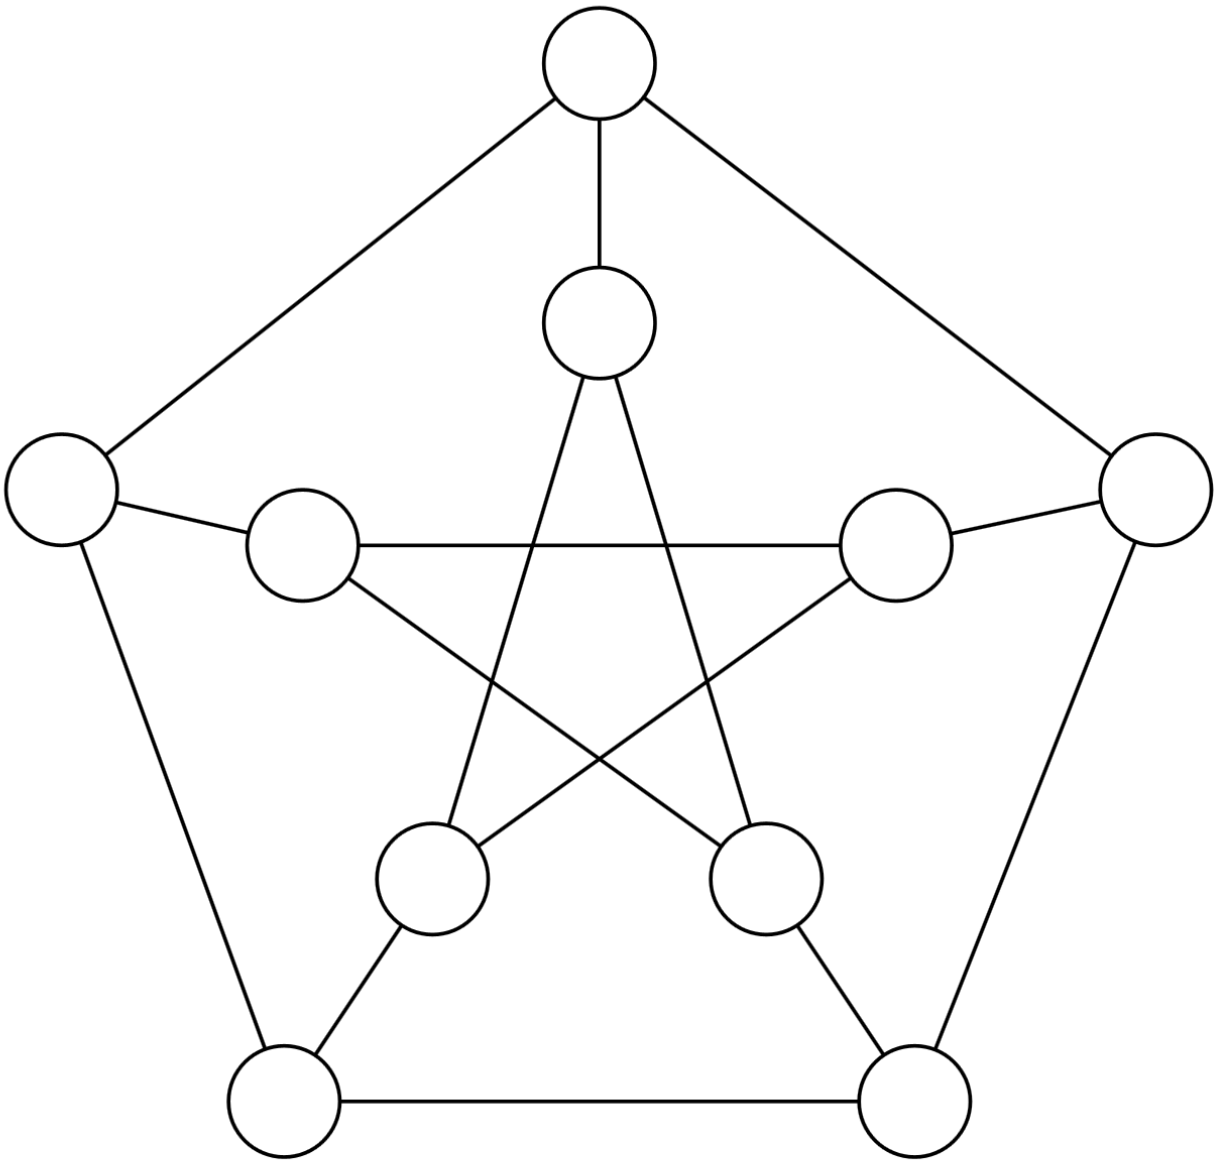
\includegraphics[height=5cm]{vertexcover1}}
		\only<all:2>{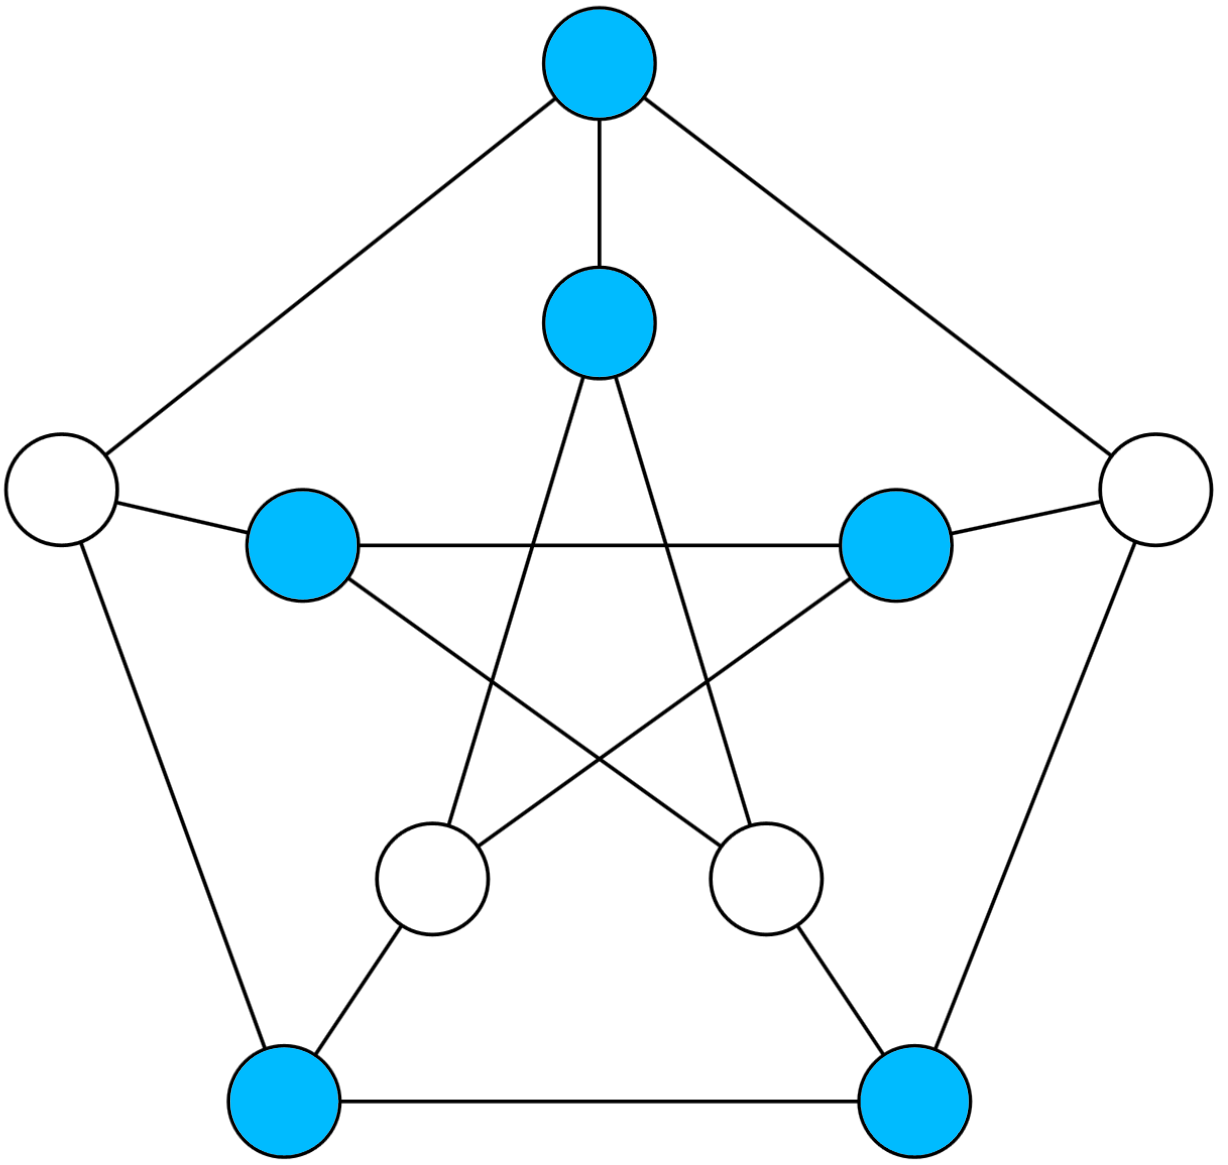
\includegraphics[height=5cm]{vertexcover2}}
	\end{figure}
\end{frame}

\begin{frame}{Optimierungsprobleme – ILPs}
	\textbf{\textsc{VertexCover} als ILP} 
	\begin{itemize}
		\item \textbf{Lösungsvektor} $x \in \{0, 1\}^n$: \quad $x_i = 1$ \gdw Knoten $i \in C$ 
		\pause
		\item Kostenvektor $c = (1,..,1) \in \{1\}^n$, \\ 
		\textbf{minimiere} $f(x) = c \cdot x = \sum x_i = |C|$
		\pause
		\item $m$ \textbf{Constraints}: \quad  $\forall \{u, v\} \in E \quad \text{ jeweils } \quad x_u + x_v \geq 1$
		\pause 
		\begin{align*}
			{\Impl} \qquad \min_{x \in \set{0,1}^n} &f(x) = c \* x \\
			\text{sodass} \quad & x_u + x_v \geq 1 \quad \forall \set{u,v} \in E \\
			\text{mit} \quad & \text{$c = (1,..,1)$.} 
		\end{align*}
	\end{itemize}
\end{frame}

\iffalse
\begin{frame}<handout:0>{Optimierungsprobleme}
	\textbf{Zusammenfassung: Was haben wir heute gelernt?} 
	\begin{itemize}
		\item Verschiedene Verfahren für das Lösen von Optimierungsproblemen: Greedy, DP, ILP
		\pause
		\item TGI wird bestimmt super
		\pause
		\item Gruppenarbeit ist \textbf{megatoll} und überhaupt das \textbf{AllerBUÄSTE} von der \textbf{ganzön Welt}, deshalb sollten wir \textbf{unbedingt} jetzt gleich eine solche machön!!!1!
	\end{itemize}
\end{frame}
\fi

\begin{frame}{Optimierungsprobleme – ILPs}
	\vspace{-.3\baselineskip}
	\taskheading{Seine Abschiedsvorstellung}
	Der ebenso geniale wie wahnsinnige Superbösewicht Doktor Meta lacht hysterisch: Die Weltherrschaft ist zum Greifen nah! Der verrückte Superschurke plant nämlich, die gesamte Welt in einer Nacht in Schutt und Asche zu legen, um anschließend eine neue Weltordnung aufzubauen. Dafür muss er lediglich ausreichend Militärdepots und sonstige explosionsgefährdete Lagerstätten in die Luft jagen. Genügend Schurken und Handlanger zu rekrutieren, die bei der Verlegung von Zündschnüren helfen, kostet allerdings viel Geld. Er will daher möglichst wenig Depots in die Luft sprengen und trotzdem die ganze Welt, also alle Planquadrate $1...k$, ausradieren. Auf der Welt gibt es insgesamt $n$ Depots, wobei ein Depot $i$ die Planquadrate $P_i \subseteq \set{1,...,k}$ dem Erdboden gleichmachen kann, was allerdings $c_i$ Euro kostet. Nun muss der Superbösewicht lediglich die billigste Menge aller Depots bestimmen, die alle Planquadrate $1...k$ abdeckt.  \\
	Helft mit, die Welt zu zerstören und formuliert das Problem als ILP.
\end{frame}

\begin{frame}{Optimierungsprobleme – ILPs}
	\solutionheading
	\begin{itemize}
		\item \textbf{Lösungsvektor} $x \in \{0, 1\}^n$, \\ 
		\§{\quad $x_i = 1$ \gdw }Depot $i$ wird zur Sprengung ausgewählt  \\
		\. (\entspr Planquadrate $P_i$ sind abgedeckt)
		\item \textbf{Kostenvektor} $c = (c_1, ..., c_n) \in \R_{\geq0}^n$ \\
		\quad Minimiere $f(x) = c \cdot x = \sum c_i x_i$
		\item $k$ \textbf{Constraints}, \quad für $j = 1...k$: \\
		\quad $\sum\limits_{i=1}^{n} P_{ij} \cdot x_i  \geq 1$ \quad mit $P_{ij} = \casesl{1, \ \text{Planquadrat } j \in P_i \\ 0, \ \text{Planquadrat } j \notin P_i}$
		\implitem Andere Schreibweise: \\
			$\min\limits_{x \in \set{0,1}^n} c \* x \quad \text{sodass} \quad P^\top \* x \geq \scalebox{.7}{$\large \Matrix{1 \\ \vdots \\ 1}$}$\!\! \quad\! mit $P = (P_{ij})$, $P_{ij} = ...$, $c = ...$ 
	\end{itemize}
	Das Problem heißt allgemein übrigens \textsc{SetCover}.
\end{frame}

\begin{frame}{Danke für eure Aufmerksamkeit! \smiley}
	\centering
	\textbf{\textsc{Travelling Salesman Problem}} \\[.2\baselineskip]
	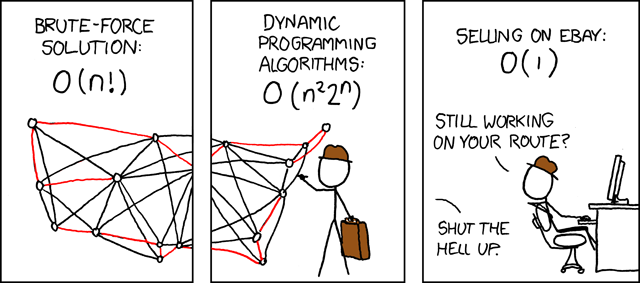
\includegraphics[width=.9\textwidth]{xkcd}
\end{frame}

\only<beamer:0>{\slideThanks}

\end{document}